\documentclass[12pt]{ociamthesis}  % default square logo 
%\documentclass[12pt,beltcrest]{ociamthesis} % use old belt crest logo
%\documentclass[12pt,shieldcrest]{ociamthesis} % use older shield crest logo

%load any additional packages
\usepackage{amssymb}
\usepackage{subfig} % Required for creating figures with multiple parts (subfigures)
\usepackage{amsmath,amssymb,amsthm} % For including math equations, theorems, symbols, etc
\usepackage{varioref} % More descriptive referencing
\usepackage{listings} %allows insertion of code with text wrapping
\usepackage{verbatim} %allows block comments
\usepackage{graphicx}
\usepackage{float}

\lstset{
basicstyle=\scriptsize\ttfamily,
breaklines=true
columns=flexible,
}
 

%input macros (i.e. write your own macros file called mymacros.tex 
%and uncomment the next line)
%\include{mymacros}

\title{Experimental observations of droplet formation and polydispersity in T-junction microfluidic devices with pressure-driven flow}   %note \\[1ex] is a line break in the title

\author{Aaron Delahanty\\
	BSc Mechanical Engineering}             %your name and qualifications
	
	
\college{School of Engineering\\[1ex]
College of Science and Engineering}  %your college


%\renewcommand{\submittedtext}{change the default text here if needed}
\degree{Master of Science}     %the degree
\degreedate{2016}         %the degree date

%end the preamble and start the document
\begin{document}

%this baselineskip gives sufficient line spacing for an examiner to easily
%markup the thesis with comments
\baselineskip=18pt plus1pt

%set the number of sectioning levels that get number and appear in the contents
\setcounter{secnumdepth}{3}
\setcounter{tocdepth}{3}


\maketitle                  % create a title page from the preamble info
%\include{dedication}        % include a dedication.tex file
%\begin{acknowledgements}
I would like to express my gratitude to Thomas Franke's group and their generosity of time, patience, and guidance. I would also like to thank the international community of University of Glasgow and the city of Glasgow as a whole for the inclusivity, openness, and willingness to accept any curious mind as its own. Let Glasgow Flourish.
\end{acknowledgements}   % include an acknowledgements.tex file
\begin{abstract}


%Background:
Microfluidic devices generally require precise control of fluid flowrates in order to accurately and reliably perform their various functions. In the case of droplet-makers fluid flow may be manipulated to dictate the size, frequency and distribution of droplets. Multiple approaches may be taken in order to control fluid flow in such devices. Here a pressure-driven flow controller (PDFC) is developed and characterized for use as a flow provider for droplet-makers and as a tool for further microfluidics-based research.

%Objectives:
	Previously, droplet-makers that utilize volumetric flow control have been used to define the relationship between continuous and discontinuous phase flowrates and the resulting droplet parameters and flow regimes. Here pressure-driven droplet-makers are characterized and compared to the existing systems.
Furthermore, an investigation into the ability to control droplet formation in real-time is conducted by quantifying the time-to-stability of the electronic flow controller and droplet-maker system.

%Methods:
The work conducted and presented here can be divided clearly into three sections (i) design, fabrication, development of the PDFC (ii) characterization of the PDFC system and (iii) investigation into the behavior of droplet-maker devices as driven by pneumatic pressure.

%Results:
	The PDFC system consists of a micro controller, sensing pressure transducers, regulating pressure transducers, as well as various pneumatic and electronic components used to integrate the system into University of Glasgow's Franke Lab's existing microfluidic test set-up. The system was characterized to show pressure control ranging from 0 to 1000mbar with 4 discreetly controlled channels capable of  precision of XX with a time response of XX. When applied as the flow controller for droplet-makers it was found that droplet formation as defined by length:width behaved similarly to previously volumetric flow rate systems.

%Limitations:
A major limitation of pressure-driven flow systems is that the flow rate within microfluidic devices varies as a function of device geometry. Herein significant discussion is presented as to methods of theoretical and experimental approximations of the volumetric flowrates resulting from pressure-driven flow.


\end{abstract}          % include the abstract

\begin{romanpages}          % start roman page numbering
\tableofcontents            % generate and include a table of contents
\listoffigures              % generate and include a list of figures
\end{romanpages}            % end roman page numbering

%now include the files of latex for each of the chapters etc
\chapter{Introduction}

The study of microfluidics requires by definition generation of fluid flow. In research and experimental environments syringe pumps are commonly used as flow providers \cite{Christopher2008}. They offer the advantage of being capable of directly controlling the rate of flow in units of volume per time. Furthermore, programmable syringe pumps have been developed that allow for modulation of flowrate as a function of time. An alternative to syringe pump systems is pressure-driven flow in which precision regulated compressed gas is used to pressurize fluid-filled reagent reservoirs, which in turn drives flow through small diameter tubing and subsequently any applicable microfluidic device. A custom developed pressure-driven flow system may offer advantages such as increased flow stability, capability to support high numbers of parallel flow channels, and flowrate modulation response time \cite{Bong2011, Lim2015}. This project focus on the development of such a system, herein referred to as a Pressure Driven Flow Controller (PDFC). 

One application of the system is the formation of micro-droplets. Micro-droplets are generally an aqueous vessel contained within an oil carrier, whose biological applications span DNA analysis, protein crystallization, and cell encapsulation. Furthermore, highly precise fluidic operations can be performed on the microscale including mixing, merging, and splitting \cite{Cristini2004}. The method and technology surrounding droplet production is relatively mature, first demonstrated by Thorson \emph{et al.} in 2001 \cite{Thorsen2001}. However, droplet production using pressure-driven flow is relatively uncharacterized and has been identified as an area in need of further investigation \cite{Christopher2008}.

The work documented here can be divided into two primary categories. First, the PDFC system is designed, built, and characterized. Secondly, the developed device is put to use to characterize micro-droplet formation in T-junction geometry operating under pressure-driven flow. This document is to be divided accordingly. First the design, development, and characterization of the flow device is presented. Followed by a presentation of the background theory necessary to discuss droplet formation. Experimental observations are presented and discussed. Finally, a conclusion is presented that describes the major accomplishments and courses of further investigation.

\chapter{System Development}

\section{Design}

System design is covered here with the intent of allowing for future modification or reproduction of the flow system. Development of neither the labVIEW Virtual Interface (VI) nor microcontroller are covered in detail but are presented in the attached appendixes. The electronics skills required to build the system include analogue and digital electronics but are of basic undergraduate level and are not covered in any detail here. 

\qquad


\paragraph{Design Inputs} High level design inputs were generated by discussion with the the research group of Thomas Franke and may be summarized as follows:


\begin{enumerate}
\item The flow system shall be controlled by a labVIEW VI.
\item The flow system shall feature four discrete pressure channels.
\item The flow system shall be capable of producing pressure output 
from 0 to 1 bar.
\item The resulting controlled pressure shall be visible to and recordable by the user.
\end{enumerate}

\clearpage

\paragraph{System Components}In order to develop a system capable of meeting these design inputs several key components are required, specified in Table \vref{tab:syscomp}

\qquad

 
\begin{table}[H]
\begin{center}
\begin{tabular}{l*{6}{c}r}
Component & Manufacturer & Part Number & Quantity \\
\hline
Regulators & Marsh Bellofram & Type 2000 & 4 \\
Transducers & AMS & 5915-1000-D & 4\\
Transducers & AMS & 5915-0350-D & 4\\
DACs & MCP & 4921 & 4\\
Microcontroller & Arduino & Uno R3 & 1 \\
\end{tabular}
\caption [Key System Components]{Key System Components} 
\label{tab:syscomp}
\end{center}
\end{table}

Alternative components may be acceptable, even superior, to those detailed here. Specifically, pressure transducers that allow for faster modulation may be sought. The time response of the system developed here is covered in Section \ref{sec:characterization}. In addition to the key components listed here other basic electrical components were required including standard off-the-shelf resistors, capacitors, molex-connectors and prototyping solderboard.

The system electronics are packaged within a IP 66/IP 67 DIN EN 60529 rated enclosure, shown in Figure \vref{fig:sysPhoto}. The system functions as a 'black box' with the 240VAC$->$9VDC power input, USB communication, main pneumatic supply line input, and 4 discrete regulated pressure outputs.

\begin{figure}[H]
\centering 
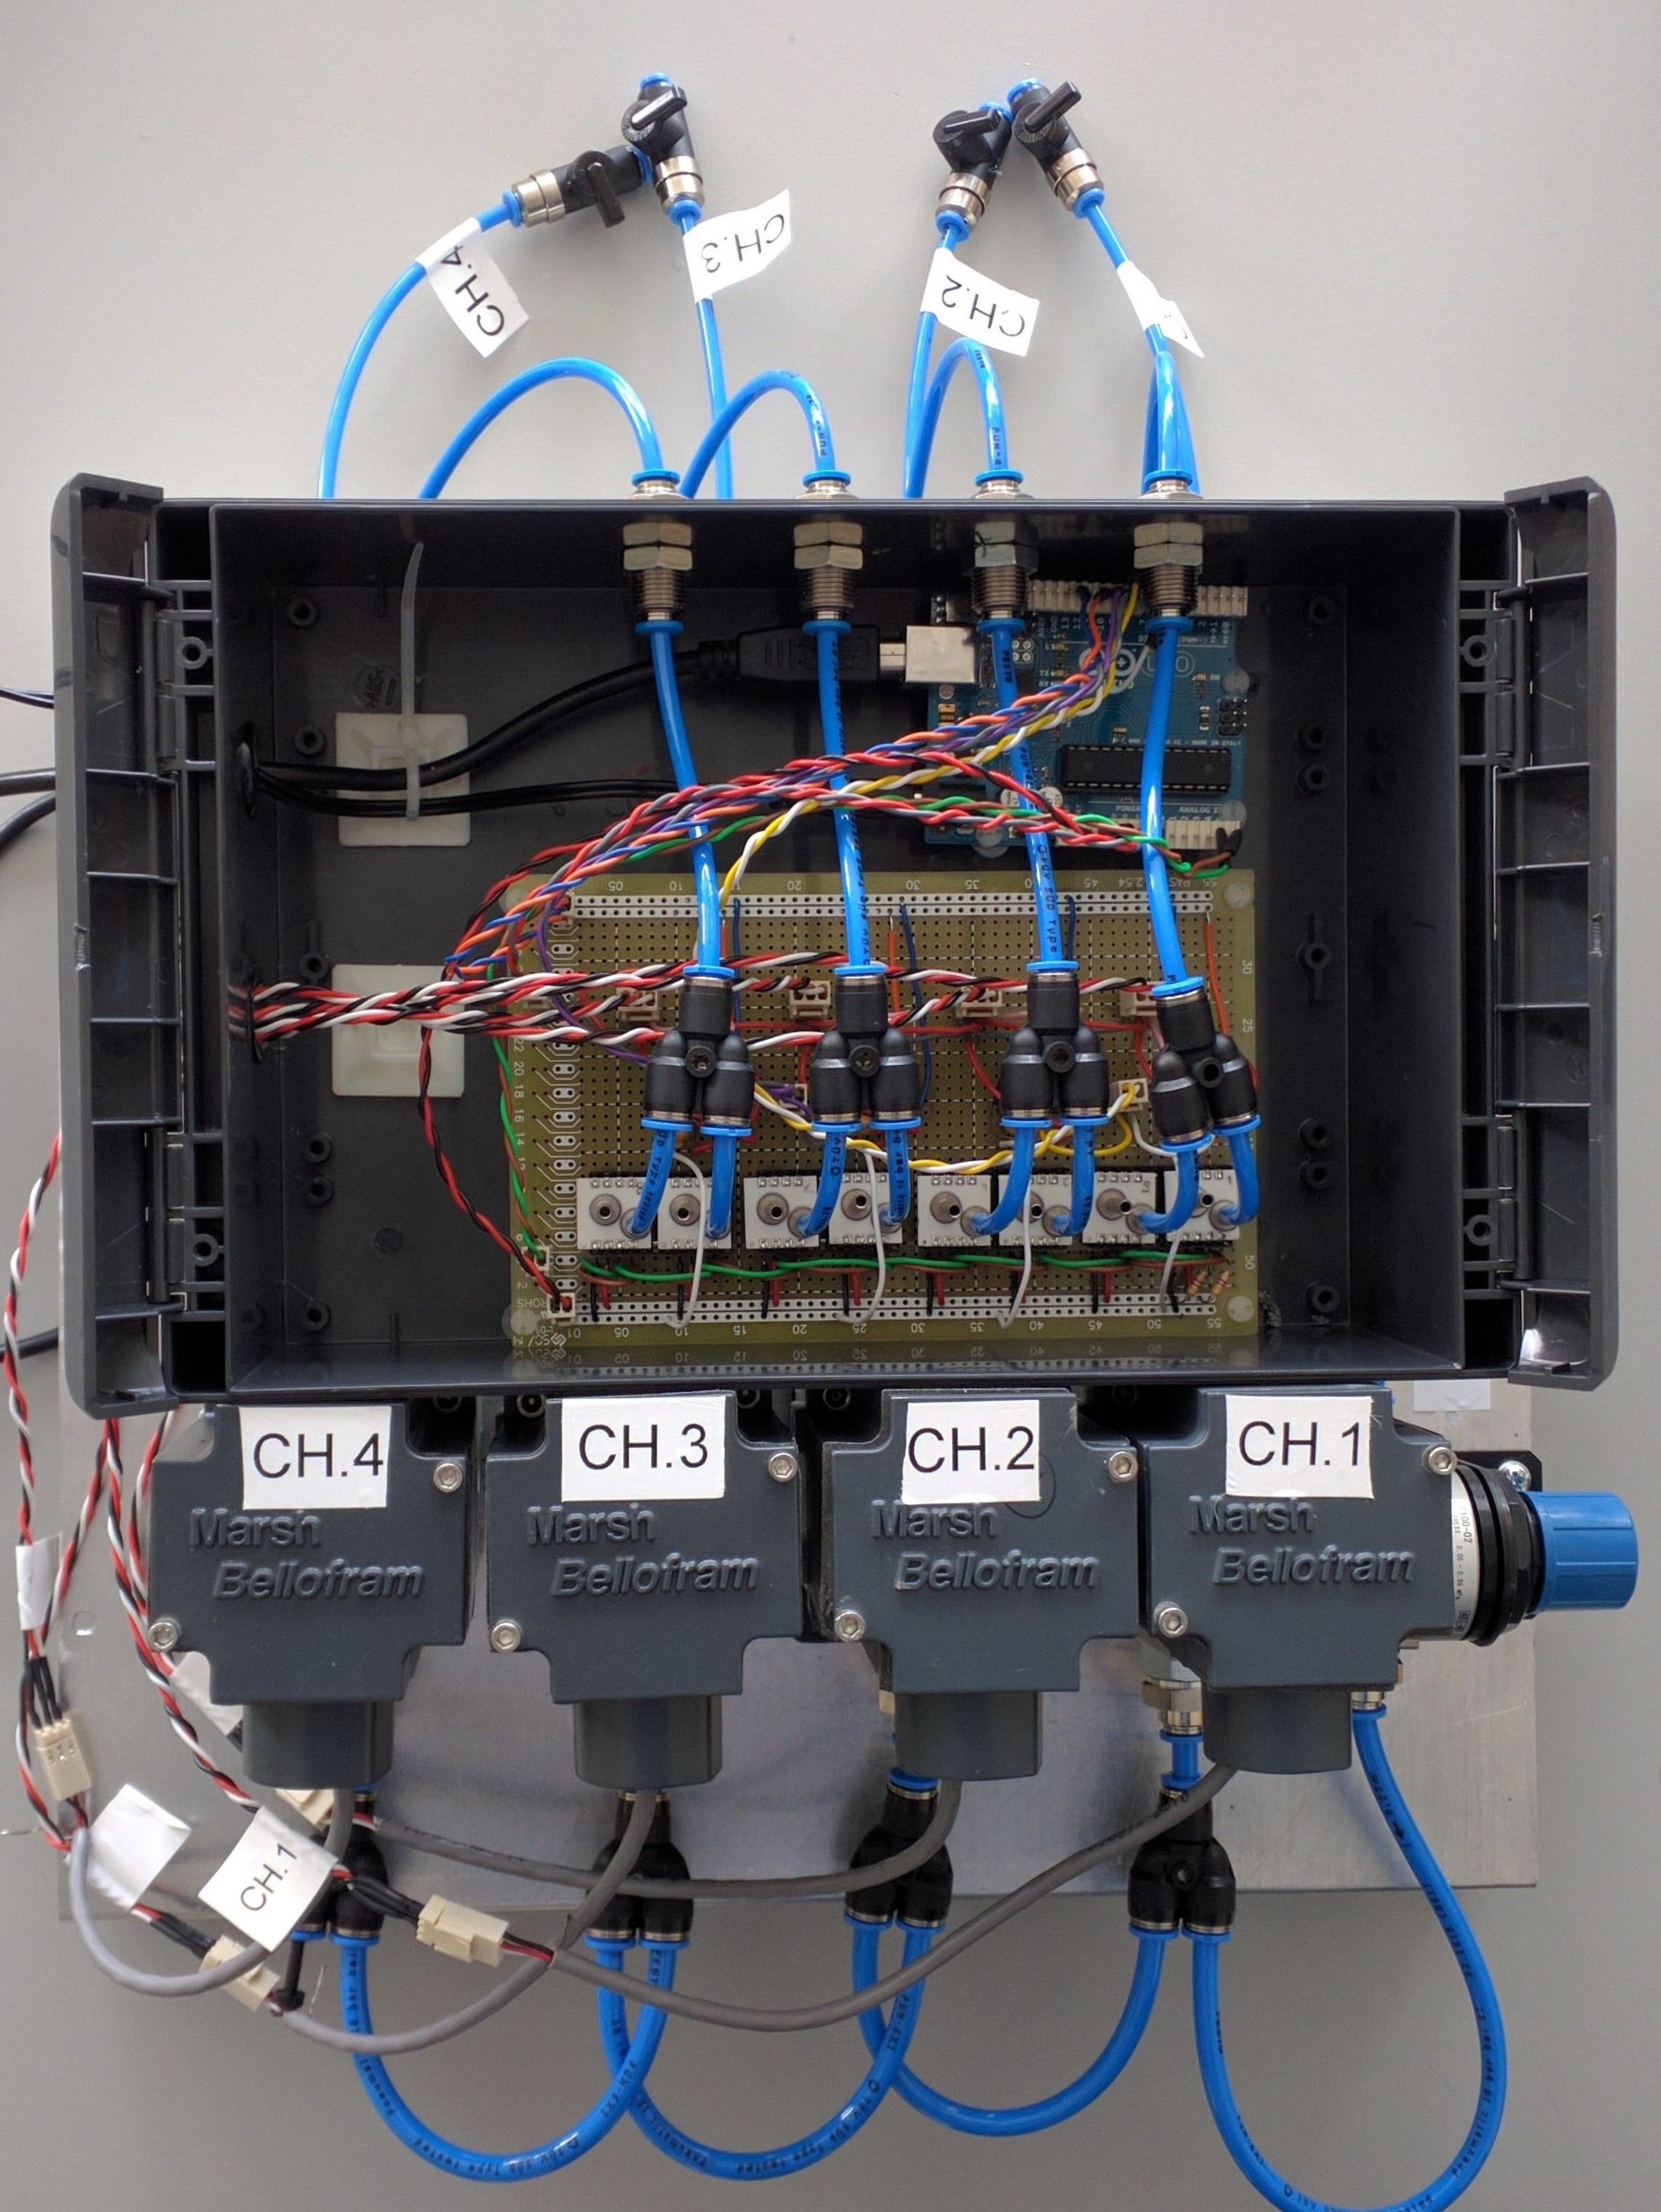
\includegraphics[width=0.750\columnwidth]{sysPhoto.PNG} 
\caption[Image of Packaged PDFC]{The PDFC as contained in the final enclosure.} 
\label{fig:sysPhoto} 
\end{figure}

Several pneumatic components are required to provide a compressed gas flow path between the supply, the regulators, transducers, and reagent reservoirs. These components are summarized in the pneumatic schematic for a single channel is shown in Figure \vref{fig:pneumaticSchematic}. Note that the air supply here is expected to be filtered to remove excess humidity and provide 3 micron particle filtration. 

\begin{figure}[H]
\centering 
\includegraphics[width=1.0\columnwidth]{pneumaticSchematic.PNG} 
\caption[Pneumatic Schematic of PDFC channel]{The pneumatic schematic detailing a single channel of the PDFC. The four primary components moving down through the schematic are the supply, T2000 pressure regulator, AMS pressure transducers, and the terminal flow reservoir.} 
\label{fig:pneumaticSchematic} 
\end{figure}

\paragraph{Operational Overview} The PDFC system is designed to be managed by interaction with a custom LabVIEW VI. The user manually enters a desired control signal within the labVIEW interface of 0 to 5 volts, corresponding to operational pressure range of 0 to 1000mbar.

\begin{figure}[H]
\centering 
\includegraphics[width=0.5\columnwidth]{writeVI.PNG} 
\caption[LabVIEW write command]{Control pressures are set digitally within the LabVIEW interface.} 
\label{fig:writeVI} 
\end{figure}

After initiating the write command the digital signal is written synchronously to the micro-controller by Universal Serial Bus (USB) via LabVIEW's 'virtual instrument software architecture'. The signal is initially sent and interpreted as a string and is processed via the embedded micro-controller code into a binary command comprised of the 4 configuration bits and 12 data bits. This binary command is then written to the digital analogue converters (DACs) via standard serial peripheral  interface (SPI) protocol. The DACs convert the binary commands into analogue voltage outputs of 0-5V. This voltage is routed to the input of each pressure regulator and results in the desired pressure output of 0 to 1000 mbar.

The controlled output of each pressure regulator is then split by a y-connector. One flow path goes to the reagent reservoir to drive fluid flow, the other is routed back into the PDFC for real-time measurement by the integrated chip pressure transducers. Each regulated pressure channel is measured by two different 14bit transducers, one is low range (0-350mbar) with increased resolution, the other is full range (0-1000mbar). The pressure transducers produce a digital signal that is then transferred back to the micro-controller via I2C protocol. Finally the measured pressures are sent to the LabVIEW VI for display and optional recording. This entire control process including LabVIEW and microfluidic device integration is summarized in system overview shown in Figure \vref{fig:systemOverview}.



\begin{figure}[H]
\centering 
\includegraphics[width=1.0\columnwidth]{systemOverview.PNG} 
\caption[System Overview of the PDFC]{The control loop used to set and measure channel pressures using the PDFC} 
\label{fig:systemOverview} 
\end{figure}

\clearpage

\section{Characterization}
\label{sec:characterization}


After completing manufacture and integration of the PDFC it must be validated prior to being used as a research tool. Particular emphasis is placed on two operating criteria of the system:
\begin{enumerate}
\item The response time of the system, from application of write signal to regulated pressure response.
\item The accuracy and channel-to-channel variance observed in the system.
\end{enumerate}

In regards to the response time of the system it may be valuable to detail the magnitude of individual response times for the process steps required from signal input to response output, summarized in Table \vref{tab:compTime}

\begin{table}[H]
\begin{center}
\begin{tabular}{l*{6}{c}r}
Process Step & Magnitude of Time Response(ms) \\
\hline
Sync. USB Comm. & 1000 \\
Arduino String $->$ Binary & 1 \\
DAC & 1\\
Pressure Regulator & 100\\
\end{tabular}
\caption [Component Response Time]{Component Response Time} 
\label{tab:compTime}
\end{center}
\end{table}

The labVIEW VI is capable of recording the measured regulated pressure outputs, which may be used to document control pressures utilized for specific experimentation. Here, that data logging capability is used to investigate the system's time response, as shown in Figure \vref{fig:timeResponse}. The gap in data is due to use of 'synchronous' USB communication within the LabVIEW environment. The rightmost data prior to the gap coincides with the time point at which the command signal is sent. While all channel outputs clearly converge to the desired nominal output pressure, the time response is broadly speaking slow, and variation in channel regulation is apparent as the pressure output stabilizes. Variation in the stabilization of regulated signal is due to differences in the control circuit from regulator to regulator. The model of regulator used here relies on a Proportional Integral Differential (PID) control circuit with manually adjustable potentiometers to adjust gain constants, non-ideal when attempting to produce coincident outputs on discrete channels.

The time from signal write to that of reaching $95\%$ of the desired output, $\tau$, increases as a function of differential pressure sought but is roughly on the magnitude of $~1 sec$. 

\begin{figure}[H]
\centering 
\includegraphics[width=01.0\columnwidth]{timeResponse.PNG} 
\caption[PDFC time response]{Three pressure transitions are shown, 40 to 80mbar, 30 to 40mbar, and 25 to 30mbar for 3 discrete output channels. } 
\label{fig:timeResponse} 
\end{figure}

These observations suggests that the system, as currently developed, is not appropriate for the millisecond or faster response times required for real-time manipulation of droplet size. This agrees with previous findings. Flow rate control of droplet formation is known for its slow response whether by syringe pump or pressure flow. Furthermore, response time of the actual device is further delayed due to fluidic capacitance caused by the compressibility of reagents, tubing and PDMS channels \cite{Churski2013,Stone2004}. If fast-response times are sought a more appropriate methodology may be to maintain a steady flowrate and drive droplet formation by active methods through direct manipulation of the fluid at the local point of formation by electrical, mechanical, magnetic, or acoustic means \cite{Chong2016}.


System accuracy and channel to channel variation can be investigated in a similar method to time response. Here, three channels are simultaneously regulated to a nominal 100mbar. After a stabilization time of approximately 3 seconds, a 15 second mean and standard deviation are acquired for each channel, as shown in area between the dashed lines in Figure \vref{fig:constV}. Each channel is capable of regulating to the nominal 100 $\pm$ 1 mbar with a standard deviation of less than 0.25 mbar. The capability to maintain stable pressure and hence steady flow is critical for production of highly monodispersed droplets, as documented in Results section \ref{sec:results}.


\begin{figure}[H]
\centering 
\includegraphics[width=01.0\columnwidth]{constV.PNG} 
\caption[PDFC accuracy and inter-channel variation]{Accuracy and channel-to-channel variation of the PDFC system.} 
\label{fig:constV} 
\end{figure}
\chapter{Background Theory}

Development of a pneumatic pressure driven flow system for use in microfluidic research requires a firm grasp on the transition from 'macro' fluidics to microfluidics. The system operates across a great range of scales drawing and compressing air from a room of several cubic meters that is subsequently used to provide flow in channels of only a few micrometers. Following the flow path of the system - compressed air is filtered and directed via large diameter $(~5mm)$ tubing to reagent columns of large diameter $(~2cm)$, where the compressed air acts on the reagent to produce flow through smaller tubing $(<1mm)$ before finally transitioning into the microfluidic device where channel dimensions are on the order of magnitude of micrometers. This range of scale is illustrated in Figure \vref{fig:systemScale}

\begin{figure}[h]
\centering 
\includegraphics[width=0.60\columnwidth]{systemScale.PNG} 
\caption[System Scales]{Illustration of the scales involved in the system.} % The text in the square bracket is the caption for the list of figures while the text in the curly brackets is the figure caption
\label{fig:systemScale} 
\end{figure}

\clearpage

The importance of forces that act on fluids therefore dramatically changes from the macro- to the microscale. With downscaling, the buoyancy, gravitational and inertial forces are less and less important and viscous and interfacial forces become more and more predominant.\cite{Shui2007}


\section{Droplet microfluidics Overview}
Phase is a distinct state of matter in a system; matter that is identical in chemical composition and physical state and separated from other material by the phase boundary. Multiphase fluids are those in which there exist at least two different fluids in a system with different chemical composi- tions ? liquid/liquid, or with different physical states ? gas/ liquid.\cite{Shui2007}. Here we neglect consideration of gas-liquid two phase systems. 


\cite{Yang2010,Shui2007a,Zhao2011}


The study of fluid dynamics requires the analysis of individual fluid forces (such as gravity, inertial, viscous, and interfacial forces) and an understanding of how these forces combine to define fluid behavior. In order to understand the transition from large dimension $(>1mm)$ to small dimension $(<1mm)$ systems it may be useful to understand how these forces relate to system dimensions by the way of scaling laws. Some fluid forces such as inertial forces and gravity forces are dependent on the \emph{volume} of fluid involved. Other fluid forces are intrinsically defined by the \emph{surface area} of the fluids such as viscous forces and interfacial forces. More broadly speaking each of various fluid forces may be dependent on the different orders of characteristic length, $l$. For example, inertial force is dependent on density, $\rho$, which may be expressed as mass per volume or mass per $l^3$, as shown in Equation \vref{eq:inertia}. Similarly, interfacial tension is often defined as the partial differential of the Gibb's free energy over area, where the area term may be expressed in terms of $l^2$, shown in Equation \vref{eq:interfacial}.


\begin{equation}
i = \rho \nu^2 = \frac{m}{V}\nu^2 = \frac{m}{(l^3)}\nu^2 
\label{eq:inertia}
\end{equation}

%Probably wont use this eqn:
%\begin{equation}
%P = \rho g h = \frac{m}{V}g h
%\label{eq:pressure}
%\end{equation}

\begin{equation}
\gamma = \frac{\partial G}{\partial A} = \frac{\partial G}{\partial (l^2)}
\label{eq:interfacial}
\end{equation}


Consider the relative effect these individual forces have on the overall fluid behavior in which the volume dependent forces have an $l^3$ term and the surface forces have a $l^2$ term, as shown in Equation \vref{eq:scalingLaw} \cite{bruus2008}

\begin{equation}
\frac{Surface Forces}{Volume Forces} \propto \frac{l^2}{l^3} = l^{-1} \lim_{l \to 0}  \rightarrow \infty
\label{eq:scalingLaw}
\end{equation}

From this comes the realization that as systems are miniaturized towards a theoretical zero-dimension the surface forces begin play an exponentially larger effect relative to the volume forces, illustrated in Figure \vref{fig:scalingLaw}.

\begin{figure}[h]
\centering 
\includegraphics[width=0.60\columnwidth]{scalingLaw.PNG} 
\caption[Law of Scales for microfluidic forces]{Illustration of the law of scales as fluid systems are miniaturized.} % The text in the square bracket is the caption for the list of figures while the text in the curly brackets is the figure caption
\label{fig:scalingLaw} 
\end{figure}

\paragraph{Navier-Stokes} Early attempts at approximating fluid flow by Bernoulli and his pupil Euler completely neglected the viscosity term (an aforementioned surface force) in their mathematical expressions. In systems of small dimensions the viscosity effects are dominant and these approximations are inadequate. The Navier-Stokes expression accommodates viscous forces and is essentially a statement of force balance between inertial, pressure and viscous forces, shown in Equation . In most microfluidic systems the inertial forces are small enough that they may be neglected and the expression reduces to the statement that the net pressure forces are equal to the negative net viscous forces \cite{Vyawahare2014}.

\begin{equation}
\rho \Bigg(\frac {\partial \nu}{\partial t} + \nu \cdot \nabla \nu \Bigg) = - \nabla P+ f +\eta \nabla^2 \nu + \nabla \sigma
\label{eq:navierStokes}
\end{equation}

\begin{equation}
\frac {\partial \nu}{\partial t} + \nabla \cdot  ( \rho \nu) = 0
\label{eq:navierCOM}
\end{equation}

\begin{equation}
\rho \frac {\partial \nu}{\partial t} = - \nabla P+ f +\eta \nabla^2 \nu + \nabla \sigma
\label{eq:navierCOM}
\end{equation}

\^ above equations from \cite{Shui2007}

\paragraph{Dimensionless Groups} In many cases fluid flow at the microscale can be best categorized by comparing \emph{dimensionless groups} driven by fluid parameters such as viscosity, velocity, density and system geometry, as is the case of the dimensionless group known as Reynold's Number \emph{(Re)} shown in Equation ~\vref{eq:reynolds} . Regardless of the specific fluid or geometric parameters, systems with similar \emph{Re}  numbers general behave similarly - making it  powerful tool in characterization of a microfluidic system. The \emph{Re} value can be described in real world terms as a relation between the inertial forces and viscosity forces at play in a system. At the microscale viscous forces are dominant over inertial forces thus the \emph{Re} value is typically very low, indicating flow is laminar \cite{Kleinstreuer2013}.

\begin{equation}
Re =\frac {\rho \nu L}{\mu}
\label{eq:reynolds}
\end{equation}

Where $\rho$ is fluid density, $\nu$ is fluid velocity, $L$ is characteristic length, and $\mu$ is fluid viscosity. The \emph{Re}  value dictates whether the system will be within the laminar or turbulent regime. \emph{Re} values tend to be small $(< 5)$ for microfluidic systems because the spatial scale, and therefore characteristic length, are small while fluid viscosity is constant relative to larger-scale systems \cite{D??azNafr??a2013}. As the majority of microfluidic systems feature small \emph{Re} numbers the dimensionless group becomes less valuable in the differentiation and categorization of different systems. \\
For water in a straight micro- or nanochannel with a diameter between 100 nm and 100 ?m, where ?(H2O)=1.025�10? 3 Pa s, ?(H2O)=103 kg m? 3 and v=1 mm s?1, the calculated Reynolds number lies between 10? 1 and 10? 4. For a gas, oxygen for instance, ?(O2)= 20.317�10? 6 Pa s and ?(O2)=1.429 kg m? 3, the Reynolds number in the same system ranges from 10?5 to 10?2. Therefore, inertial forces are overwhelmed by interfacial forces in microfluidic devices, and laminar flow is expected in micro- and nanochannels, and not turbulent or random flow\cite{Shui2007}.\\
Other dimensionless groups such as Capillary Number, Peclet Number,  Viscosity Ratios, Flowrate Ratios are commonly used to describe microfluidic systems - specifically droplet-producing geometries such as the device inestigater in section 'asdafs'. \cite{DeMenech2008}

The Capillary number \emph{(Ca)} is a dimensionless group that compares the relative contribution of interfacial forces and viscous forces. The capillary number is especially useful in discussion of two-phase microfluidic systems because it neglects any inertial forces and is capable of describing droplet formation behavior as influenced by solution viscosity and surface energies.  The \emph{Ca} is defined as shown in Equation \vref{eq:ca} \cite{D??azNafr??a2013}.

\begin{equation}
Ca =\frac {\mu u}{\gamma}
\label{eq:ca}
\end{equation}

Where $\mu$ is defined as the viscosity of the continuous phase, $u$ is the mean fluid velocity, and $\gamma$ is the interfacial tension between the discontinuous and continuous phases. The viscous forces and interfacial forces determining fluid behavior are generally understood to act tangentially and normal to the two-phase interface, respectively. Viscous forces along the droplet surface work in elongation of surface of the droplet where as interfacial forces work to minimize the interfacial are. These two opposing behaviors when acting in different ratios dictate the droplet behavior as categorized by the different fluid regimes dripping, squeezing, jetting(XX?)\cite{Shui2007}.

\section{Hydrodynamic Resistance}

\begin{figure}[h]
\centering 
\includegraphics[width=01.0\columnwidth]{resistanceSystem.PNG} 
\caption[Hydraulic Resistance of System]{The microfluidic system detailed from the reagent water column to the waste reservoir.} % The text in the square bracket is the caption for the list of figures while the text in the curly brackets is the figure caption
\label{fig:resistanceSystem} 
\end{figure}


$\Delta P = R_{HYD} Q$

$Q_1 = Q_2 = Q_3 = Q_4$



$R_{HYD} = R_1 + R_2 + R_3$

$R_1 = R_3 = \frac{8 \eta L}{\pi r^4}$

$R_2 = \frac{28.4 \eta L}{ h^4}$



For the purpose of quantifying the contribution to total pressure drop of the droplet-maker relative to the inlet and outlet tubing the following values were applied to first solve for the flowrate at an arbitray pressure of 500mbar. Assuming that $P_4$ is equivalent to atmospheric pressure, 0 Pa, and $L_1 = 0.100m$, $L_2=0.001m$, $n=1cP = 0.001 Pa-s$, $r=0.0025m$ and $h=0.000030m$. Take $P_1 = 500mbar = 50kPa$ which is mid operational range for the system.


$R_1 = R_3 = \frac{8 (0.001) (0.100)}{\pi 0.0025^4} = 6.52  \times 10^6 \frac{kg}{m^4s}$

$R_2 = \frac{28.4 (0.001) (0.001)}{ 0.000030^4} = 3.51 \times 10^{13}\frac{kg}{m^4s}$

Clearly the resistance seen over the length of the simplified droplet-maker is several orders of magnitude greater than the resistance of the input/output lines. The total pressure $(P_4 - P_1)$ is known (it is the command pressure of the PDFC) and the individual pressure differentials can be calculated as follows:
\\

$P_4 - P_1 = (2 (\frac{8 \eta L_1}{\pi r^4}) + \frac{28.4 \eta L_2}{ h^4}) Q$
\\

First solving for the flowrate:
\\
\\
$Q = \frac{P_4 - P_1 }{(2 (\frac{8 \eta L_1}{\pi r^4}) + \frac{28.4 \eta L_2}{ h^4})}$
\\
\\
$Q = \frac{50,000} {(2 (6.52*10^6) + 3.51*10^{13})} = 1.42  \times 10^{-9} \frac{m^3}{s} $
\\
\\
$Q =  1.42*10^{-9} \frac{m^3}{s}  \times  \frac{1000 L}{m^3} = 1.42  \times 10^{-6} \frac{L}{s}$ 

Assuming that the system is at steady state and therefore the microfluidic structure (tubing and PDMS) is not expanding due to internal pressure we can infer that by conservation of mass and assumed incompressible fluids that the volumetric flowrate is constant across each of the system pressure points shown in Figure ~\vref{fig:resistanceSystem}. We can then produce the following system of equations:
\\
$P_2 - P_1 = (R_1) Q$
\\
$P_3- P_2 = (R_2)Q$
\\
$P_4 - P_3 = (R_3) Q$
\\
Applying the previously calculated resistances and flowrate the following pressure differentials are obtained:
\\
$P_2 - P_1 = 9.26 \times 10^{-3 }\frac{kg}{m \cdot s^2} =  9.26 \times 10^{-3} Pa$
\\
$P_3- P_2 = 49.84 \times 10^{3 }\frac{kg}{m \cdot s^2} =  49.84 \times 10^{3} Pa$
\\
$P_4 - P_3 = 9.26 \times 10^{-3 }\frac{kg}{m \cdot s^2} =  9.26 \times 10^{-3} Pa$
\\

At these values (and given these are all simple linear equations this should be the case regardless of flow viscosity, etc.) the pressure drop across the micro-scale device comprises of:

$\frac{P_3-P_2}{P_4-P_1} = \frac{49.84 \times 10^{3}}{50.00 \times 10^{3}} = 0.9968$

And so it may be appropriate to neglect the pressure drops across the tubing and assume that the PDFC applied pressure is equivalent to the pressure applied across the droplet-maker. This can be further justified by the fact that the control precision of the system (a few mbar) is larger than the negligible pressure differentials of the tubing sections. XX consider modeling this using the same modeling software used for the BD lab (especially modeling the pressure drops across the microfluidic device itself.




\chapter{System Application - Droplet Microluidics}
\section{Aims}
The application of the PDFC to droplet microfluidics serves two purposes. First, it verifies that the system is functioning as intended for use as a practical research tool. Second, it allows the characterization of droplet formation by a pressure driven flow in T-junction geometry, an area currently underdeveloped \cite{Christopher2008}. 

\section{Methods}
\subsection{Device Generation}

The T-junction microfluidic device referenced herein is fabricated using standard soft lithography methods \cite{Stroock2002}. Two part Polydimethylsiloxane (PDMS) was poured onto a SU-8 mold previously developed by Schmid and Franke \cite{Schmid2014c} to form an array of individual $25 \mu m \times 25 \mu m$ T-junction channels. The PDMS was cured at 65dC for 3 hours. After cooling to room temperature, the set PDMS was cut and removed from the mold. Tubing connection holes were punched using a standard $0.5mm$ biopsy punch. Next, a standard glass slide and the PDMS channels are oxygen-plasma treated, adhered, and exposed to 100dC for 1hour. Prior to use, devices are treated with the aquapel for 10mins, purged with filtered compressed gas and dried at 65dC for 3 hours. 

\subsection{Reagents}

Reagents were formulated in bulk, the same formulation was used for all data presented here. The continuous phase consists of 3M's HFE-7500 fluorocarbon oil stabilized with fluorosurfactant ammonium carboxylate DuPont Krytox 157 to concentration of 2.0 wt\% . This discontinuous phase consists of de-ionized water and Sigma Aldrich's B0126-256 Bromophenol blue, dissolved in 0.1M NaOH, to a final concentration of 1mM.

\subsection{Experimental Procedure}

The microfluidic device was installed on an upright microscope with 20X Objective and brightfield illumination. Images are acquired by Photon fastcam at 500 frames per second (fps). The devices were first primed with the oil phase to preferentially wet the channel walls prior to introduction of the aqueous phase. The applied control pressure was held constant for the continuous phase while varying the discontinuous phase control pressure to achieve varying flow conditions. Discontinuous phase control pressure was varied at intervals no smaller than $\approx$5mbar until droplet formation ceased due to the onset of backflow or instability, for low or high pressures, respectively. 

\subsection{Analysis of Collected Data}

The captured images were then analyzed using a custom imageJ script, shown in Figure \vref{fig:imageJ}. The script differentiates the droplets from the carrier fluid to determine droplet length, $L$,  position, $X$, along an arbitrarily defined axis parallel to the geometry's outlet channel and the frame at which the measurement occurs.

\begin{figure}[H]
\centering 
\includegraphics[width=01.0\columnwidth]{imageJ.PNG} 
\caption[Custom ImageJ Droplet Analysis Script]{Custom imageJ script used to isolate and measure droplets.} 
\label{fig:imageJ} 
\end{figure}


\section{Results}
\label{sec:results}

\subsection{Regime Transition}

For the T-junction channel geometry described, the dimensionless droplet ratio of droplet length, $L$, over channel width, $W$, is plotted as a function of the applied control pressure ratios, $\frac{P_{H_2O}}{P_{Oil}}$, shown in Figure \vref{fig:lwvpr}. Error bars have been calculated by standard deviation of measured droplet length which results in error equal to or smaller than the symbol size and thus not shown. Linear regression models have been applied to the data points expected to be within the squeezing regime. The slopes of the fitted lines were determined as 3.909, 4.151, and 5.370 for applied continuous phase pressures of 40, 60, and 80 mbar with coefficients of determination of 0.958, 0.996, and 0.990, respectively. Full summary statics of the linear regression fit are presented in the Supplementary Statistics Appendix.

\begin{figure}[H]
\centering 
\includegraphics[width=01.0\columnwidth]{lwvpr.PNG} 
\caption[Droplet Length as a Function of Applied Control Pressure Ratio]{Standard (left) and log-log (right) plots of droplet length as a function of the applied control pressure ratio for T-junction geometry. Note the distinct change in slope as the pressure ratio increases, an indication of regime transition.} 
\label{fig:lwvpr} 
\end{figure}

Outer Ca values are calculated given an interfacial tension of $\gamma = 2.87 \times 10^{-3}\frac{N}{m}$ (as measured by spinning method), continuous phase viscosity of $\mu = 1.24 \times 10^{-3} Pa \cdot s$\cite{3M2009}, and mean velocity, $u$, as determined by droplet position over consecutive frames.

Droplet length is plotted as a function of capillary number as shown in Figure \vref{fig:regimes2} for each of the applied continuous pressures. The critical capillary numbers were approximated as 0.0135, 0.0185, and 0.0215 for 40, 60 and 80 mbar continuous phase pressures, respectively. Images of droplet formation are shown within the squeezing and dripping regimes for each continuous phase control pressure. The images shown are captured one frame prior to droplet formation. 

\begin{figure}[H]
\centering 
\includegraphics[width=0.75\columnwidth]{regimes2.PNG} 
\caption[Droplet length as a function of Capillary number across squeezing and dripping regimes]{Top: Droplet length as a function of Capillary number across squeezing and dripping regimes. The transition between dripping and squeezing regimes is marked by vertical dashed lines, corresponding to critical capillary numbers of 0.0135, 0.0185, and 0.0215. Bottom: Typical images of droplet elongation just prior to formation.} 
\label{fig:regimes2} 
\end{figure}

\clearpage

\subsection{Droplet Polydispersity}

Variance in droplet dimensions is analyzed by evaluating the length of droplets formed by constant applied control pressures. Images were acquired at 500 fps for a period of 10 seconds resulting in a sample size of at least 100 droplets with at least three length measurements taken in subsequent frames per unique droplet. A variety of plots investigating population statistics are shown in Figure \vref{fig:1_poly}, for data acquired at $P_{OIL} = 20mbar,  P_{H_2O} = 80mbar$, resulting in a $Ca$ value of 0.010. The same analysis was conducted at two higher $Ca$ values and is found in the Supplementary Statistics Appendix .

\begin{figure}[H]
\centering 
\includegraphics[width=0.90\columnwidth]{1_poly.PNG} 
\caption[Polydispersity]{Population distribution of droplet length for $P_{oil} = 0.1 bar, Ca = 0.010$. Top-left: Mean droplet length as shown by measured X-position. Top-right: Droplet length shown over the duration of image acquisition. Bottom-left: Histogram of measured droplet length. Bottom-right: Q-Q plot for the droplet length population.} 
\label{fig:1_poly} 
\end{figure}

\clearpage

From the analyzed data, droplet velocity, flowrate, capillary number, mean length, length standard deviation and percent Coefficient of Variation are extracted. A summary of the resulting dimensional statistics is shown in Table \vref{tab:poly}.

\qquad

\begin{table}[H]
\begin{tabular}{l*{6}{c}r}
$ P_{Ratio} $ & $ V_C  (m/s) $ &  $ Q_C ( \mu  L/min) $ & Ca & $ Mean Length( \mu m )$ & $ StdDev( \mu m) $ & C.V. \\
\hline
4 & 0.023 & 0.863 & 0.010 & 57.71 & 0.55 & 0.95 \\
2.25 & 0.033 & 1.238 & 0.014 & 54.53 & 0.35 &  0.64 \\
1.66 & 0.043 & 1.613 & 0.018 & 48.14 & 0.21 &  0.43 \\
\end{tabular}
\caption[Droplet Polydispersity]{Dimensional analysis of droplets}
\label{tab:poly} 
\end{table}


\clearpage


\section{Discussion}
\subsection{Droplet Regime Transition}

Previous work has been done to establish specific flow regimes in which droplets are formed in T-junction geometry by both numeric modeling and experimental investigations \cite{Abate2012a, DeMenech2008, Garstecki2006}. Previous findings suggest that two stable droplet formation regimes exist in T-junction droplet formation, \emph{dripping} and \emph{squeezing}. In a highly cited paper, De Menech et al showed by numerical modeling that the transition between the two distinct droplet regimes may be defined by a Critical Capillary Number, $Ca_{cr}$, and that this transition is independent of viscosity ratio and flowrates. This transition has been previously determined both experimentally and in numerical simulations to be $Ca_{cr}\approx 10^{-2}$ \cite{Christopher2008, DeMenech2008, Xu2008}. These values of Capillary Numbers represent a threshold below which the interfacial forces significantly dominate the viscous forces. Thus, in these geometries, the discontinuous phase is only minimally elongated as it enters the T-junction and instead extends orthogonally to the main channels such that the channel is plugged prior to droplet formation. After the droplet blocks the channel outlet, break-up proceeds driven by the building pressure differential due to the blockage.

\begin{comment}
\begin{figure}[H]
\centering 
\includegraphics[width=0.75\columnwidth]{menechtransition.PNG} 
\caption[Menech Regime Transition]{Used directly, without permision} 
\label{fig:menechtransition} 
\end{figure}
\end{comment}

\emph{While the regime transition has been well documented through numerical simulations and in experiments utilizing volumetric-flow, to the best of the author's knowledge there has been no record of experimental observations demonstrating the regime transition from squeezing to dripping in a pressure-driven flow system.} This, despite the fact that there have been documented dissimilarities in volumetric versus pressure-driven flow in droplet formation\cite{Ward2005}, and that there may be advantages in droplet monodispersity in pressure-driven systems \cite{Christopher2008,Li2014a}.

The data presented here shows a distinct transition between dripping and squeezing regimes, as demonstrated by the change in slope shown in Figure \vref{fig:lwvpr}. The plot shows a transition from dripping regime to squeezing regime as the pressure ratio increases. The squeezing regime appears to be linear as determined by the linear regression models. This linearity agrees with Gastecki's findings that within the squeezing regime droplet L/W is a function of only the channel geometry, represented by the $\alpha$ coefficient, and the  volumetric flowrates, $Q_{in} $and $ Q_{put}$ shown in Equation \vref{eq:garstecki} \cite{Garstecki2006}.

\begin{equation}
L/W = 1 + \alpha Q_{in} / Q_{out}
\label{eq:garstecki}
\end{equation}

Here, L/W data is presented as a function of applied pressure ratios rather than flowrate ratios and therefore cannot be directly compared. Furthermore, the data presented here exists precisely at the transitional capillary numbers and therefore contains droplets formed within both regimes as opposed to Garstecki's purely squeezing regime data. Therefore, in order to draw further conclusions regarding droplet dimensions as they pertain to flow ratios in a pressure-driven system both these complications must be overcome. 

The transition between regimes may also be shown by the changing behavior of droplet length as a function of capillary number shown in Figure \vref{fig:regimes2}. However, the critical capillary number at which the transition occurs is not universal between the varying flowrates as shown previously \cite{DeMenech2008}. The transitional capillary number can be plotted as a function of the continuous phase pressure as shown in Figure \vref{fig:CrCaABline}.

\begin{figure}[H]
\centering 
\includegraphics[width=0.75\columnwidth]{CrCaABline.PNG} 
\caption[Critical capillary number as a function of continuous phase applied pressure]{Critical capillary number as a function of continuous phase applied pressure.} 
\label{fig:CrCaABline} 
\end{figure}

The difference in critical capillary number is likely due to the use of droplet velocity as an approximation for mean continuous phase velocity. Others have surmised that there is some numerical difference between the velocity of the droplets and the mean velocity of the continuous phase \cite{Ward2005}. Unfortunately, due to the complex nature of multiphase flow during droplet formation it may be difficult to further investigate the true mean velocity of the continuous phase. However, a correction can be made by applying the linear relationship between the applied control pressure of the continuous phase and the critical capillary number such that the regime transition is coincident, as shown in Figure \vref{fig:ca_cor}. 

\begin{figure}[H]
\centering 
\includegraphics[width=0.750\columnwidth]{ca_cor.PNG} 
\caption[Droplet Length as a function of Corrected Capillary Number]{Droplet length as a function of corrected capillary number. The dashed vertical line shows the interpreted point of transition.} 
\label{fig:ca_cor} 
\end{figure}

This interpretation of droplet length as a function of corrected critical capillary number is a simplification that clearly demonstrates the regime transition. However, it should be noted that these capillary numbers have first been approximated, then linearly scaled, and that a systematic investigation in which flowrates are calculated by varying methods should be conducted to understand the effect on capillary number approximation.
\clearpage

\subsection{Droplet Polydispersity}

Dimensional analysis of droplet length shows there is no statistically meaningful difference in droplet length as measured at varying points as the droplet migrates down the channel. Additionally, there does not appear to be any strong trend in measured droplet length over the duration of image acquisition. Both histograms and Quantile-Quantile plots of the mean droplet length suggest the populations to be largely normal. 

Polydispersity in syringe pump based systems suffers, particularly at low flow velocities, due to minor fluctuations in the stepper-motor-actuated syringe plungers \cite{Christopher2008}. Here, polydispersity is measured by the coefficient of variation (CV) on the population’s droplet length. In the populations measured, the CV was below 1\%. This is significantly lower than the 6 to 10\% CVs reported by experimental observations in T-junctions using syringe pumps at similar flowrates \cite{Christopher2008}. The results are similar to the polydispersity reported by others using pressure-driven flow. However, the CVs shown here suggest this system is capable of marginally improved monodispersity relative to the $~2\%$ CVs reported elsewhere and at even lower flowrates \cite{Kaminski2016, Lim2015}. The lowest continuous phase flowrate droplet population measured here was 0.863 $\mu $L/min, resulting in a capillary number of $0.010$ and CV of $0.95$.


\chapter{Conclusions}


\section{Areas of Further Investigation}

Given the nature of the PDFC as a general flow provider and that it is intended to be used for applications outside of droplet formation there are systems aspects that may be improved.

\subsection{Improvement of Time Response}
It may be beneficial to seek faster actuating regulators and to improve the signal propagation time (currently limited by the LabVIEW VISA tool set). One approach may be to move pressure control signal generation to the microcontroller and to use LabVIEW as a tool only to set parameters that drive specific time-dependent functions on the micro-controller. Similarly, the microcontroller could be interacted with directly, bypassing the need for LabVIEW integration all together by use of custom inputs. It is also important for future users to consider that compressibility of the system will have an impact on the response time.

\subsection{Determination of Flowrate}
One of the limitations of the system is the determination of flowrates. Multiple methods of flowrate determination have been described here, including droplet velocity, mass measurement, and hydraulic resistance approximation. Each of these methods has some drawback that makes application difficult. It is conceivable that imageJ (or similar) image analysis could be used to develop a tool capable of automatically determining flowrates and would be valuable for a broad range of applications.

\clearpage

\section{Achievements}
This project was divided into two primary objectives. First, to develop and characterize a pressure driven flow controller system for use as flow provider in microfluidic applications. Second, the system was applied to the generation of droplets using a T-junction microfluidic device.

\subsection{Device Development}

The PDFC system was successfully integrated into the existing microfluidic laboratory set-up. The initial design inputs were all fulfilled as demonstrated by the presented system characterization. The system was shown to have a response time on the order of magnitude of approximately 1000ms, significantly faster than comparable syringe pump based systems \cite{Bong2011}. The resulting regulated pressures were shown to be very stable with low inter-channel variation. The PDFC was measured to be capable of $\pm$ 1 mbar accuracy with a signal standard deviation of less than 0.25 mbar, and signal to noise ratio of 400. This highly stable pressure results in high stable flowrates given the system is allowed to come to steady-state, and therefore in the application of droplet formation produces high monodispered droplets.

\subsection{Application to Droplet Formation}
The PDFC was subsequently used to produce droplets at low capillary numbers in T-junction micro-channels. The transition between flow regimes was established, shown in Figures \vref{fig:lwvpr} and \vref{fig:regimes2}. While the parameters and conditions resulting in droplet-formation regime transition have been well documented by others, this, to the best of the authors knowledge, is the first time the transition has been experimentally documented in a pressure-driven flow system. The transition was quantified by the outer capillary number, and was found to be 0.0135, 0.0185, and 0.0215 for the three different continuous phase pressures tested, similar to values previously reported \cite{Christopher2008,DeMenech2008}. However, unlike previous findings the critical capillary number was not shown to be universal across multiple flow conditions. This may be due to the approximation of the continuous phase mean velocity as calculated from the measured droplet velocity. 

The droplets produced were highly monodisperse in normally distributed populations, with droplet length coefficient of variations of less than 1\%. This level of monodispersity was considerably improved relative to syringe pump based systems, and similar to monodispersity achieved by others using similar systems\cite{Kaminski2016, Lim2015}.


%now enable appendix numbering format and include any appendices
\appendix
\chapter{Arduino Code}
\scriptsize

\begin{lstlisting}

    
//Aaron Delahanty
//2224135D@student.gla.ac.uk
//University of Glasgow
//21Oct2015
//Electronic Flow Controller

//This application (sketch) is intended to be the sole sketch responsible for measuring 
//and regulating pressure in the Electronic Flow Control (EFC) system being developed 
//for T.Franke's microfluidic group. The objective of the sketch is to faciliate
//communication with two types of integrated chips (i) Analog Microselectronic's AMS5915
//pressure sensors,and (ii) Microchip Technology Inc.'s MCP4921 DAC.

//In addition to this sketch the system will use a LabView VI to set the desired 
//pressure values by DAC, and display the measured pressure for the 4 discrete channels
//This communication will be facilated by serial communication over USB.

//Revision Notes:
//02192016  - Removed Volmeter functionality
//          - Removed All Delays
//          - 4th Channel DAC is faulting (output is always 1V)


//Wire.h is the arduino library for I2C/TWI comm
#include <Wire.h>
#include <SPI.h>

//Define variables used for conversion of pressure units from raw counts mbar.
    int p_min;
    int p_max;
    int digoutp_min;
    int digoutp_max;

//Define array for pressure channel comaprison and final output
//Comparison is used to determine whether the high range 1000mbar or high resolution 
//350mbar sensor should be used
    float p_comp[8];
    float p_out[4];

//Prior to sending the 12bit input which will drive the T2000 pressure regulators
//the DAC needs to receive 4 configuration bits
//Bit 15 - 0 = write to DAC, 1 = ignore command
//Bit 14 - BUF; 1 = buffer v_ref, 0 = bypass buffer
//Bit 13 - GA; 1 = v_out is 1X v_ref, 0 = vout is 2X v_ref
//Bit 12 - SHDN; 1 = active, 0 = shutdown DAC

//Default configuration bits set to [0,1,1,1]
    unsigned int Config = B0111;

void setup()
{
    //Set baud rate to 9600 
    Serial.begin(9600);
    // join i2c bus
    Wire.begin(); 
    // join SPI bus
    SPI.begin();
}

void loop()
{

//START DAC CODE:

 // check serial 

  if ( Serial.available() ){
    // cast the string read in an integer 
    String p_write = Serial.readString();

  int commaIndex1 = p_write.indexOf(',');
  int commaIndex2 = p_write.indexOf(',',commaIndex1+1);
  int commaIndex3 = p_write.indexOf(',',commaIndex2+1);


  String P1s = p_write.substring(0,commaIndex1);
  String P2s = p_write.substring(commaIndex1+1,commaIndex2);
  String P3s = p_write.substring(commaIndex2+1,commaIndex3);
  String P4s = p_write.substring(commaIndex3+1);

  unsigned int a[3];
  a[0]=P1s.toInt();
  a[1]=P2s.toInt();
  a[2]=P3s.toInt();
  a[3]=P4s.toInt();


    float cs[3];
    for (int i = 0; i <= 3; i++)
       {
        cs[i] = i+7;
        pinMode(cs[i], OUTPUT);
        

        
        //Command is the variable sent to DAC to drive pressure regulator
        //The commmand variable is comprised of the 4 configuration bits and 12 data bits
        unsigned int command;
        //Shift the config bits 12 positions leftward, augment with the a[i] pressure value 
        //in volts
        command = ( Config << 12 | a[i]);

        //Write command to each ith DAQ
        SPI.beginTransaction(SPISettings(20000000, MSBFIRST, SPI_MODE0));
        //Set ith output pin to LOW, in order to accept write command
        digitalWrite(cs[i], LOW);
        //SPI.transfer function is only capable of sending 8bits at a time
        //The 16bit command is therefore split into a high and low byte
        int high = highByte(command);
        int low = lowByte(command);
        SPI.transfer(high);
        SPI.transfer(low);
        SPI.endTransaction();
        //Set ith pin HIGH to end write command
        digitalWrite(cs[i], HIGH);
        //Optional print for debugging
        //Serial.println("16bit command sent:");
        //Serial.println(value,BIN);
        }
  }


//END DAC CODE

//START PRESSURE SENSOR CODE:

  //Define buffer to hold sampled values
  byte buffer[4];


  for (int addr = 1; addr <= 8; addr++)
    {
        //Pressure sensor addresses have been configured to 1 through 8.
        //Sensors 1,2,3,4 are high range 1000mbar
        if (addr <= 4)
          {
            //Set conversion constants for AMS 5915-1000-D
            p_min = 0;
            p_max = 1000;
            digoutp_min = 1638;
            digoutp_max = 14745;
          }

        //Sensors 5,6,7,8 are high resolution 350mbar
        else
          {
            //Set conversion constants for AMS 5915-350-D-B
            p_min = 0;
            p_max = 350;
            digoutp_min = 1638;
            digoutp_max = 14745;
          }

        //Wire.requestFrom(address, quantity)
        //address: the 7-bit address of the device to request bytes from
        //quantity: the number of bytes to request
        //request four bytes from sensor (first 2 are pressure, second 2 are temp)
        int n = Wire.requestFrom (addr, 4);
    
        //Ensure response is 4byte
        if(n == 4)
          {
          
            Wire.readBytes (buffer, 4);
        
            unsigned int p_raw = word (buffer[0], buffer[1]);     // word(high,low)
            unsigned int t_raw = word (buffer[2], buffer[3]);
        
            // note that the next bit operations works best with "unsigned int", not with "int"
            p_raw &= 0x3FFF;    // 14bits pressure data
            t_raw >>= 5 ;       // 11bits temeperature data, shift them in position
        
            
            // convert raw pressure to mbar (equation and constants from datasheet)
            float pressure = ((( (float) p_raw - digoutp_min ) / ((digoutp_max - digoutp_min) / (p_max - p_min ))) + p_min );
        
            // convert raw temperature to degC (equation and constants from datasheet)
            float temperature = (( (float) t_raw * 200.0 ) / 2048.0 ) - 50.0;
        
            // with the pressure comparison array with all sensor's outputs
            p_comp[addr-1] = pressure;
          }

        //If no response is present, or response is not 4bytes
        else
          {
          Serial.println ("Error, no sensor found");
          }
    }

      
   int i;
   for (i = 0; i <= 3; i++)
     {
        if (p_comp[i]> 350) 
          {
            p_out[i] = p_comp[i];
          }
        else 
          {
           p_out[i] = p_comp[i+4];
          }
        Serial.println(p_out[i]);
     }
// END PRESSURE SENSOR CODE

}
    \end{lstlisting}


\chapter{LabVIEW VI}

\begin{figure}[h]
\centering 
\includegraphics[width=01.0\columnwidth]{frontend.PNG} 
\caption[LabVIEW Frontend]{LabVIEW Frontend} 
\label{fig:frontend} 
\end{figure}

\begin{figure}[h]
\centering 
\includegraphics[width=01.0\columnwidth]{backend1.PNG} 
\caption[LabVIEW Backend True]{LabVIEW Backend} 
\label{fig:backend1} 
\end{figure}

\begin{figure}[h]
\centering 
\includegraphics[width=01.0\columnwidth]{backend2.PNG} 
\caption[LabVIEW Backend False]{LabVIEW Backend} 
\label{fig:backend2} 
\end{figure}

\chapter{Polydispersity Analysis}

\begin{figure}[H]
\centering 
\includegraphics[width=01.0\columnwidth]{2_poly.PNG} 
\caption[Polydispersity at CA = 0.014]{Polydispersity at CA = 0.014} 
\label{fig:2_poly} 
\end{figure}

\begin{figure}[H]
\centering 
\includegraphics[width=01.0\columnwidth]{3_poly.PNG} 
\caption[Polydispersity at CA = 0.018]{Polydispersity at CA = 0.018} 
\label{fig:3_poly} 
\end{figure}



%next line adds the Bibliography to the contents page
\addcontentsline{toc}{chapter}{Bibliography}
%uncomment next line to change bibliography name to references
%\renewcommand{\bibname}{References}
\bibliography{refs}        %use a bibtex bibliography file refs.bib
\bibliographystyle{plain}  %use the plain bibliography style

\end{document}

